\documentclass{article}

\usepackage[preprint]{neurips_2025}

\usepackage[utf8]{inputenc}
\usepackage[T5]{fontenc}
\usepackage[vietnamese,english]{babel}
\usepackage[hypertexnames=false]{hyperref}
\usepackage{url}
\usepackage{booktabs}
\usepackage{amsfonts}
\usepackage{nicefrac}
\usepackage[protrusion=false]{microtype}
\usepackage{xcolor}
\usepackage{graphicx}
\usepackage{float}
\usepackage{multirow}
\usepackage{array}
\usepackage{enumitem}
\usepackage{caption}
\usepackage{tabularx}
\usepackage{float}
\raggedbottom
\setlength{\parskip}{1pt}
\setlength{\textfloatsep}{5pt}
\setlength{\floatsep}{4pt}
\setlength{\intextsep}{4pt}
\setlist{nosep,leftmargin=1.25em}
\captionsetup{font=small,skip=2pt}


\title{Báo cáo Vòng 1 Datathon 2026 --- The Gridbreakers\\
\large Phần 2: Trực quan hóa \& Phân tích dữ liệu \\
\large Phần 3: Dự báo doanh thu}

\author{%
  Đội Nevergiveup \\
  Trần Nguyễn Thế Nhật \quad Nguyễn Thành Đạt \quad Phạm Huỳnh Bảo Đại \\
  \texttt{nhatjames24.2004@gmail.com}
}

\begin{document}

\maketitle

\begin{abstract}
Báo cáo này trình bày kết quả phân tích dữ liệu và mô hình dự báo doanh thu cho Datathon 2026 Vòng 1. Ở Phần 2, chúng tôi tổng hợp các phát hiện kinh doanh chính từ dashboard, bao gồm tính mùa vụ của doanh thu, hiệu quả danh mục sản phẩm, chất lượng kênh thu hút khách hàng, và các vấn đề vận hành liên quan đến hoàn trả. Ở Phần 3, chúng tôi xây dựng pipeline dự báo daily \texttt{Revenue} và \texttt{COGS} bằng ensemble các mô hình cây tăng cường, Ridge regression, calibration và giải thích mô hình bằng SHAP. Kết quả cho thấy mô hình nắm bắt tốt các tín hiệu mùa vụ, xu hướng sau 2020 và chu kỳ trong tháng, đồng thời tạo ra file nộp đúng định dạng để hỗ trợ lập kế hoạch tồn kho, khuyến mãi và vận hành.
\end{abstract}


\section{Giới thiệu}
Dự án sử dụng bộ dữ liệu thương mại điện tử ngành thời trang của Datathon 2026, gồm các bảng \emph{danh mục} (sản phẩm, khách hàng, khuyến mãi, địa lý), \emph{giao dịch} (đơn hàng, chi tiết đơn, thanh toán, vận chuyển, hoàn trả, đánh giá), \emph{phân tích} (huấn luyện doanh số, mẫu nộp bài) và \emph{vận hành} (tồn kho, lưu lượng web). Phần 2 chuyển dashboard \texttt{part2.pdf} thành một câu chuyện kinh doanh tuân thủ rubric (mô tả → chẩn đoán → dự báo → khuyến nghị). Phần 3 dự báo daily \texttt{Revenue} và \texttt{COGS}. Tiền xử lý chuẩn hóa ngày tháng, nối thuộc tính sản phẩm vào cấp giao dịch, và sinh các chỉ số phái sinh (gross margin, return rate, fill rate, stockout rate, delivery latency, promo usage) để hỗ trợ diễn giải.

\section{Phần 2: Trực quan hóa và phân tích dữ liệu}

\subsection{Tóm tắt điều hành}
Phần 2 cho thấy ba thông điệp rõ ràng. Thứ nhất, doanh nghiệp có quy mô đáng kể nhưng khả năng sinh lời chỉ ở mức trung bình, với \textbf{16.43 tỷ} doanh thu, \textbf{14.16 tỷ} giá vốn hàng bán, và biên lợi nhuận gộp khoảng \textbf{14\%}. Thứ hai, hiệu quả kinh doanh không đồng đều giữa các tháng, kênh bán hàng và danh mục sản phẩm, cho thấy tăng trưởng đang tập trung ở một số khu vực nhất định thay vì diễn ra rộng khắp. Thứ ba, thất thoát có thể tránh được chủ yếu đến từ hiệu quả kênh còn yếu, mức độ tập trung cao vào một số danh mục và các đơn hoàn trả liên quan đến kích cỡ.

\subsection{Chủ đề phân tích 1: Xu hướng doanh thu và tính mùa vụ}

\begin{figure}[htbp]
    \centering
    \begin{minipage}[t]{0.48\linewidth}
        \centering
        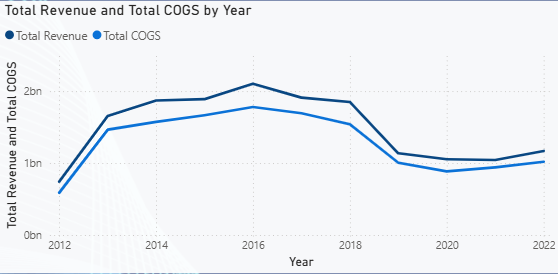
\includegraphics[width=\linewidth]{figures/year_revenue_cogs.png}
    \end{minipage}
    \hfill
    \begin{minipage}[t]{0.48\linewidth}
        \centering
        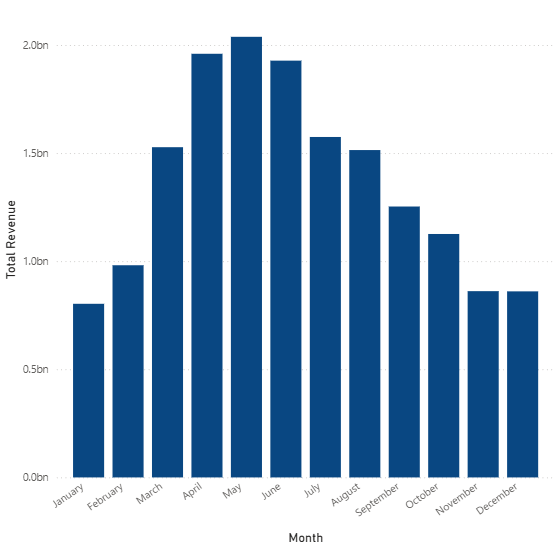
\includegraphics[width=\linewidth]{figures/monthly_revenue.png}
    \end{minipage}
    \caption{Mô hình doanh thu theo thời gian. Doanh thu năm và giá vốn hàng bán biến động khá sát nhau, trong khi doanh thu theo tháng cho thấy đỉnh mùa vụ rõ rệt vào giữa năm.}
    \label{fig:seasonality}
\end{figure}

Doanh thu thể hiện tính mùa vụ rõ ràng. Doanh số tăng từ tháng Một, đạt đỉnh vào khoảng \textbf{tháng Năm}, duy trì mức cao trong giai đoạn \textbf{tháng Tư--tháng Sáu}, sau đó giảm dần về \textbf{tháng Mười Một--tháng Mười Hai}. Vì doanh thu và giá vốn hàng bán biến động sát nhau, các giai đoạn cao điểm cần được quản lý cẩn thận để bảo vệ biên lợi nhuận, không chỉ tập trung vào sản lượng bán ra.

Doanh nghiệp nên lập kế hoạch tồn kho, nhân sự và chiến dịch marketing xoay quanh các tháng cao điểm lặp lại, đồng thời theo dõi sát biên lợi nhuận trong các giai đoạn này.

\subsection{Chủ đề phân tích 2: Hiệu quả sản phẩm, danh mục hoặc phân khúc}

\begin{figure}[htbp]
    \centering
    \begin{minipage}[t]{0.48\linewidth}
        \centering
        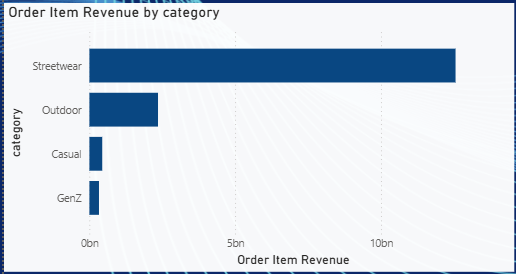
\includegraphics[width=\linewidth]{figures/revenue_by_category.png}
    \end{minipage}
    \hfill
    \begin{minipage}[t]{0.48\linewidth}
        \centering
        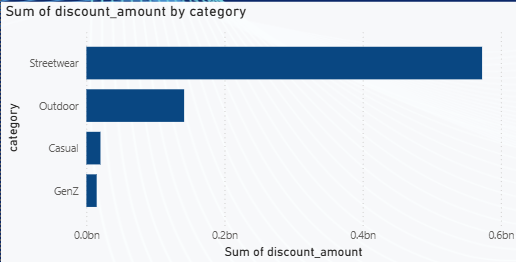
\includegraphics[width=\linewidth]{figures/discount_by_category.png}
    \end{minipage}

    \vspace{0.8em}

    \begin{minipage}[t]{0.48\linewidth}
        \centering
        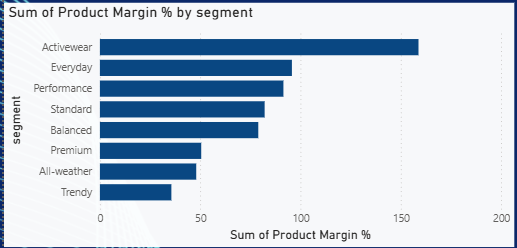
\includegraphics[width=\linewidth]{figures/margin_by_segment.png}
    \end{minipage}
    \hfill
    \begin{minipage}[t]{0.48\linewidth}
        \centering
        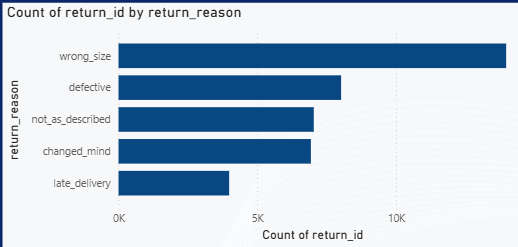
\includegraphics[width=\linewidth]{figures/returns_by_reason.png}
    \end{minipage}
    \caption{Insight về sản phẩm và danh mục. Streetwear chiếm ưu thế về doanh thu và mức chiết khấu, Activewear dẫn đầu về biên lợi nhuận, còn hoàn trả do sai kích cỡ là vấn đề hoàn trả lớn nhất.}
    \label{fig:category-performance}
\end{figure}

Cơ cấu sản phẩm có mức độ tập trung cao. \textbf{Streetwear} chiếm ưu thế cả về doanh thu lẫn chiết khấu, trong khi \textbf{Activewear} cho thấy hồ sơ biên lợi nhuận tốt nhất. Ở chiều ngược lại, \textbf{sai kích cỡ} là lý do hoàn trả lớn nhất, khiến độ chính xác về kích cỡ trở thành một vấn đề thương mại quan trọng.

Doanh nghiệp nên giảm phụ thuộc vào một danh mục duy nhất, kiểm soát cường độ chiết khấu và cải thiện hướng dẫn chọn kích cỡ để giảm các đơn hoàn trả có thể tránh được.

\subsection{Chủ đề phân tích 3: Hiểu biết về khách hàng và kênh}

\begin{figure}[htbp]
    \centering
    \begin{minipage}[t]{0.58\linewidth}
        \centering
        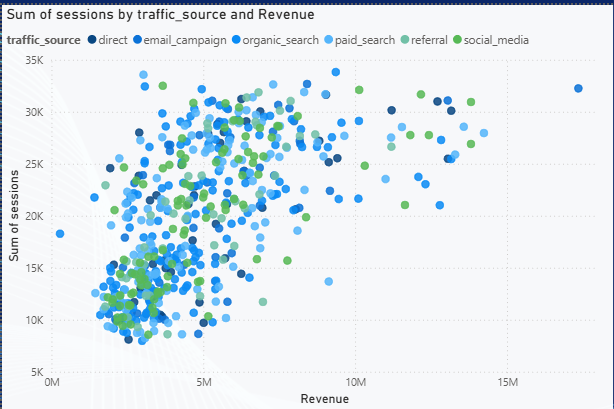
\includegraphics[width=\linewidth]{figures/channel_sessions_revenue.png}
    \end{minipage}
    \hfill
    \begin{minipage}[t]{0.38\linewidth}
        \centering
        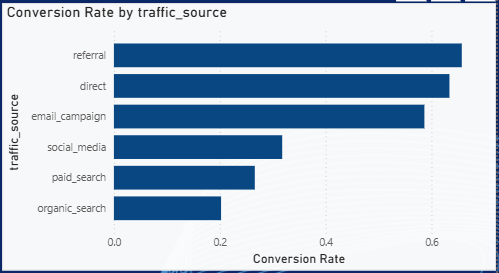
\includegraphics[width=\linewidth]{figures/channel_conversion.png}
    \end{minipage}
    \caption{Hiệu quả kênh. Lưu lượng truy cập và doanh thu có quan hệ dương nhưng không ổn định, trong khi kênh giới thiệu và truy cập trực tiếp có tỷ lệ chuyển đổi cao nhất.}
    \label{fig:channels}
\end{figure}

Chất lượng lưu lượng truy cập khác biệt rõ rệt giữa các nguồn. \textbf{Kênh giới thiệu} và \textbf{kênh trực tiếp} có tỷ lệ chuyển đổi tốt nhất, trong khi \textbf{tìm kiếm tự nhiên} và \textbf{tìm kiếm trả phí} yếu hơn. Nhiều phiên truy cập hơn không phải lúc nào cũng tạo ra doanh thu tăng tương ứng.

Ngân sách marketing nên được chuyển dịch sang các kênh có tỷ lệ chuyển đổi cao, đồng thời các kênh yếu hơn cần được cải thiện về khả năng nhắm mục tiêu và chất lượng trang đích.

\subsection{Chủ đề phân tích 4: Vận hành, giao hàng và hoàn trả}
Phần lớn doanh thu đến từ các sản phẩm không khuyến mãi, cho thấy nhu cầu nền tảng vốn đã mạnh. Hoàn trả chủ yếu đến từ \textbf{sai kích cỡ} và các vấn đề liên quan đến chất lượng. Hoạt động vận hành nên tập trung vào hướng dẫn chọn size tốt hơn, thông tin sản phẩm chặt chẽ hơn và phân bổ tồn kho thông minh hơn để giảm lost sales và các đơn hoàn trả có thể tránh được.

\subsection{Tóm tắt}
Tóm lại, bộ dữ liệu nhấn mạnh bốn ưu tiên: quản lý tính mùa vụ tốt hơn, giảm phụ thuộc quá mức vào Streetwear, đầu tư vào các kênh thu hút khách hàng có chất lượng cao hơn, và cắt giảm hoàn trả liên quan đến kích cỡ thông qua việc cải thiện truyền thông về sản phẩm và độ vừa vặn.


\section{Phần 3: Dự báo doanh thu}

\subsection{Bài toán và kiểm soát rò rỉ dữ liệu}
Task 3 yêu cầu dự báo daily \texttt{Revenue} cho giai đoạn \texttt{2023-01-01}--\texttt{2024-07-01}; file nộp cũng giữ cột \texttt{COGS} theo đúng format Kaggle. File cuối \texttt{part3/outputs/submissions/submission\_final.csv} có 548 dòng, giữ nguyên thứ tự \texttt{sample\_submission.csv}. Pipeline chỉ dùng \texttt{sales.csv} đến \texttt{2022-12-31}, không dùng target của test, không random split, và không ghép thêm chuỗi ngoài như thời tiết, vĩ mô hay thị trường.

\subsection{Quy trình mô hình hóa}
Mỗi ngày được mã hóa bằng khoảng 88 đặc trưng: calendar (tháng, thứ, đầu/cuối tháng, payday), Fourier cycles cho mùa vụ năm/tuần/tháng, event flags (11/11, 12/12, Black Friday, Tết), promotion windows từ \texttt{promotions.csv}, và regime/trend features sau 2020. Hai target \texttt{Revenue}, \texttt{COGS} được học trên thang \texttt{log1p}. Validation là hold-out cuối chuỗi: train đến \texttt{2022-07-04}, validate đến \texttt{2022-12-31} (180 ngày), nên calibration không nhìn thấy tương lai.

Kiến trúc là ensemble bốn lớp: (1) LightGBM, XGBoost, CatBoost và LightGBM Quantile-50, mỗi booster gồm base model và 4 quarterly specialists; (2) Ridge regression trên feature chuẩn hóa z-score; (3) blend $20\%$ Ridge và $80\%$ GBM blend; (4) calibration theo từng target. Pipeline giữ hai artifact: \texttt{submission.csv} là biến thể tốt nhất trên validation, còn \texttt{submission\_final.csv} là bản fixed-calibrated dùng để nộp Kaggle.

\begin{table}[H]
\centering
\caption{Cấu hình rút gọn của mô hình và chiến lược huấn luyện}
\label{tab:model_config_summary}
\renewcommand{\arraystretch}{1.25}
\begin{tabularx}{\linewidth}{p{0.26\linewidth} X}
\hline
\textbf{Thành phần} & \textbf{Cấu hình} \\
\hline

LGB 
& Learning rate $=0.016$, \texttt{num\_leaves} $=127$, $\lambda_2 = 1.0$. \\

LGB-Q50 
& Learning rate $=0.03$, \texttt{num\_leaves} $=63$, $\alpha=0.5$. \\

XGB 
& Objective \texttt{reg:absoluteerror}, learning rate $=0.03$, depth $=6$. \\

CAT 
& Loss MAE, learning rate $=0.05$, depth $=6$, \texttt{l2\_leaf} $=3.0$. \\

Ridge 
& $\alpha=3$, huấn luyện trên z-score features. \\

Sample weighting 
& Trọng số giai đoạn 2014--2018 là $1.0$; các năm khác là $0.01$, tức giảm $100\times$. \\

Quarterly specialist 
& Trọng số quý đích được nhân $2.0$; blend với $\alpha=0.60$. \\

Two-layer blend 
& $0.20 \times$ Ridge $+\,0.80 \times$ GBM. \\

Booster blend -- Revenue 
& $0.30 \times$ LGB $+\,0.30 \times$ XGB $+\,0.15 \times$ CAT $+\,0.25 \times$ LGB-Q. \\

Booster blend -- COGS 
& $0.45 \times$ LGB $+\,0.20 \times$ XGB $+\,0.15 \times$ CAT $+\,0.20 \times$ LGB-Q. \\

Calibration 
& Revenue: $C_R=1.26$; COGS: $C_C=1.32$. \\

Seed 
& Seed $=42$. \\

Hyperparameter tuning 
& Tinh chỉnh trên fold cuối: train $\leq$ 2022-07-04, validate $>$ 2022-07-04, sử dụng Optuna với 25 trial cho mỗi cặp booster $\times$ target. \\

\hline
\end{tabularx}
\end{table}

\subsection{Kết quả và file nộp bài}
Test labels bị ẩn trên Kaggle nên MAE/RMSE/$R^2$ của test không tính được local. Bảng~\ref{tab:task3-validation} báo cáo hai biến thể trên hold-out 2022-H2: (a) \emph{auto-tuned} là calibration được Optuna chọn trực tiếp trên hold-out, (b) \emph{fixed-calibration} là bản dùng $C_R=1.26$, $C_C=1.32$ và là file thật sự nộp Kaggle.

\begin{table}[htbp]
    \centering
    \caption{Hiệu suất validation hold-out 2022-H2 của hai biến thể calibration.}
    \label{tab:task3-validation}
    \small
    \setlength{\tabcolsep}{4pt}
    \begin{tabular}{llrrr}
        \toprule
        Biến thể & Target & MAE $\downarrow$ & RMSE $\downarrow$ & $R^2$ $\uparrow$ \\
        \midrule
        \multirow{2}{*}{Auto-tuned (\texttt{submission.csv})}
            & Revenue & 444,198 & 600,258 & 0.759 \\
            & COGS    & 405,869 & 535,932 & 0.725 \\
        \midrule
        \multirow{2}{*}{Fixed-calibration (\texttt{submission\_final.csv})}
            & Revenue & 732,778 & 932,900 & 0.419 \\
            & COGS    & 764,395 & 964,759 & 0.109 \\
        \bottomrule
    \end{tabular}
\end{table}

Auto-tuned variant đạt val MAE thấp hơn rõ rệt nhưng \emph{không} là bản nộp Kaggle. Lý do: hold-out 2022-H2 nằm sát chuỗi train post-COVID phẳng, nên Optuna chọn $C_R \approx C_C \approx 1.0$ và over-fit vào level cục bộ; trong khi test 2023-2024 xảy ra sau giai đoạn phục hồi và có level cao hơn. Fixed multipliers $1.26 / 1.32$ kế thừa từ thực nghiệm calibration công khai cho đúng dạng dữ liệu này; chúng tăng val MAE nhưng \textbf{transfer tốt hơn lên test} và đem lại public leaderboard \textbf{681,610}. Dự báo trung bình là \textbf{4.20 triệu} \texttt{Revenue} và \textbf{3.75 triệu} \texttt{COGS}; tất cả đều clip không âm trước khi xuất file. Chúng tôi không ép \texttt{COGS} $\le$ \texttt{Revenue} vì trong train khoảng \textbf{10\%} ngày có \texttt{COGS} vượt doanh thu thuần (do discount/hoàn trả làm giảm net revenue), nên ràng buộc đó sẽ làm méo phân phối thực tế.

\subsection{Giải thích mô hình, tái lập và bài học}
SHAP trên tree models (Hình~\ref{fig:task3-shap}) cho thấy mô hình dựa chủ yếu vào mùa vụ, trend sau 2020, chu kỳ trong tháng và lịch campaign; các feature quan trọng nhất gồm \texttt{cos\_y1}, \texttt{t\_days}, \texttt{t\_years}, \texttt{doy}, \texttt{days\_to\_eom}, \texttt{month}, \texttt{day}, \texttt{dow}. Toàn bộ pipeline tại \url{https://github.com/NhtJm/nevergiveuppteam}; tái lập bằng \texttt{cd part3 \&\& pip install -r requirements.txt \&\& python run.py train}. Seed cố định 42; CatBoost dao động khoảng 1--2K MAE.

\begin{figure}[htbp]
    \centering
    \begin{minipage}[t]{0.42\linewidth}
        \centering
        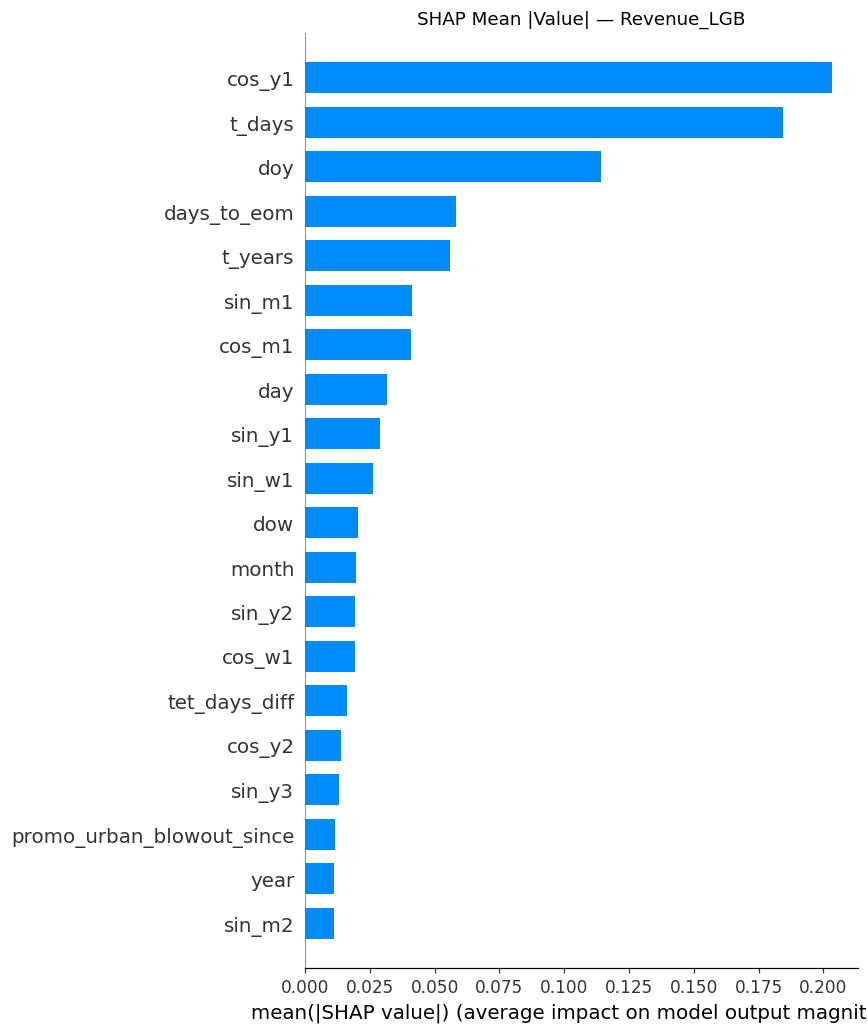
\includegraphics[width=\linewidth]{figures/shap_bar_Revenue_LGB.png}
    \end{minipage}
    \hfill
    \begin{minipage}[t]{0.42\linewidth}
        \centering
        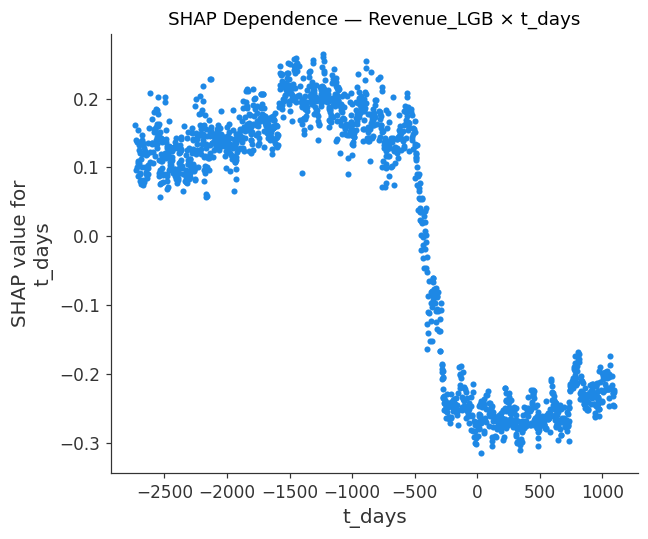
\includegraphics[width=\linewidth]{figures/shap_dep_Revenue_LGB_t_days.png}
    \end{minipage}
    \caption{SHAP cho Revenue model: feature importance và tác động của trend hậu 2020.}
    \label{fig:task3-shap}
\end{figure}

\vspace{9.5em}
\textbf{Bài học rút ra.} 5 ý tưởng giảm leaderboard score và đã bị loại: (i) \emph{recursive forecasting} với lag-1..30 — sai số tích lũy qua 548 ngày khiến mean trôi xuống, phải scale $\times$3; (ii) \emph{multi-seed averaging} ($\ge$3 seed) — làm mượt đỉnh Tết và 11/11; (iii) \emph{CatBoost depth-10 (Optuna)} — over-fit hold-out, kém depth 6 trên test; (iv) \emph{Tet-aligned lag} — xung đột sample weighting 2014--2018; (v) \emph{decomposition} $\mathrm{Rev}{=}\mathrm{orders}{\times}\mathrm{AOV}$ — pred-corr $\approx 0.985$ nên blend không tăng diversity. Insight chính: val 2022-H2 không đại diện cho test 2023-2024, fixed calibration $1.26/1.32$ khái quát tốt hơn auto-tuned, và feature mới phải vetted bằng leaderboard chứ không chỉ val MAE.\\

\section{Kết luận}
Bài làm cho thấy bốn ưu tiên hành động: chuẩn bị tồn kho trước peak demand, giảm phụ thuộc vào Streetwear, chuyển marketing budget sang kênh chuyển đổi tốt hơn, và giảm hoàn trả do sai kích cỡ. Forecasting pipeline bổ sung lớp ra quyết định định lượng cho demand planning, giúp doanh nghiệp kết nối insight EDA với kế hoạch tồn kho, campaign và logistics.

\clearpage
\section*{Tài liệu tham khảo}
\small
\begin{enumerate}[leftmargin=1.5em]
    \item Ban tổ chức Datathon 2026. \textit{Đề thi Vòng 1: Datathon 2026 --- The Gridbreakers}. VinTelligence, VinUni DS\&AI Club, 2026.
    \item Guolin Ke, Qi Meng, Thomas Finley, Taifeng Wang, Wei Chen, Weidong Ma, Qiwei Ye, and Tie-Yan Liu. LightGBM: A Highly Efficient Gradient Boosting Decision Tree. \textit{NeurIPS}, 2017.
    \item Tianqi Chen and Carlos Guestrin. XGBoost: A Scalable Tree Boosting System. \textit{KDD}, 2016.
    \item Liudmila Prokhorenkova, Gleb Gusev, Aleksandr Vorobev, Anna Veronika Dorogush, and Andrey Gulin. CatBoost: unbiased boosting with categorical features. \textit{NeurIPS}, 2018.
    \item Scott M. Lundberg and Su-In Lee. A Unified Approach to Interpreting Model Predictions. \textit{NeurIPS}, 2017.
    \item Fabian Pedregosa et al. Scikit-learn: Machine Learning in Python. \textit{Journal of Machine Learning Research}, 2011.
    \item Takuya Akiba, Shotaro Sano, Toshihiko Yanase, Takeru Ohta, and Masanori Koyama. Optuna: A Next-generation Hyperparameter Optimization Framework. \textit{KDD}, 2019.
\end{enumerate}

\end{document}
